\subsection{Projections}\label{ssec:projections}

It is sometimes important to find the component of a vector in a
particular direction. Consider the following picture:
\begin{center}
  \begin{tikzpicture}[scale=0.8,rotate=13]
    \draw[draw=green!50!black] (3,0.5) -- (2.5,0.5) -- (2.5,0);
    \draw[->, thick, red](0,0) -- node[left]{$\vect{v}$} (3,3.5);
    \draw[->, thick, blue](0,0) -- node[below, near end]{$\vect{u}$} (8,0);
    \draw[dashed] (3,3.5) -- (3,0);
    \draw[fill](0,0) circle [radius=2.25pt] node[below=1ex]{$0$};
    \draw[fill](3,0) circle [radius=2.25pt] node[below=1ex]{$P$};
    \draw[fill](3,3.5) circle [radius=2.25pt] node[right=1ex]{$Q$};
  \end{tikzpicture}
\end{center}
Here, $\vect{u}$ is a non-zero vector specifying a {\em direction},
and $\vect{v}$ is any vector. We have given the label $Q$ to the tip
of $\vect{v}$. The point $P$ lies at the place along $\vect{u}$ that
is closest to $Q$, or equivalently, such that $(0,P,Q)$ forms a right
triangle. The distance from $0$ to $P$ (measured positively in the
direction of $\vect{u}$) is called the \textbf{component}%
\index{component!of a vector}\index{vector!component} of $\vect{v}$ in
the direction of $\vect{u}$, and is denoted
$\comp_{\vect{u}}(\vect{v})$. The vector $\longvect{0P}$ is
called the \textbf{projection}\index{projection!vector to
  vector}\index{vector!projection of} of $\vect{v}$ onto $\vect{u}$,
and is denoted $\proj_{\vect{u}}(\vect{v})$. We wish to find
formulas for these quantities.

Let $\theta$ be the included angle between $\vect{v}$ and
$\vect{u}$. From trigonometry, considering the right triangle
$(0,P,Q)$, we know that
\begin{equation*}
  \cos \theta = \frac{|0P|}{|0Q|} = \frac{|0P|}{\norm{\vect{v}}},
\end{equation*}
and therefore
\begin{equation}\label{eqn:component-1}
  |0P| = \norm{\vect{v}} \cos \theta.
\end{equation}
On the other hand, from Proposition~\ref{prop:dotproduct-angle},  we
have
\begin{equation*}
  \vect{u}\dotprod \vect{v}=\norm{\vect{u}} \norm{\vect{v}} \cos \theta,
\end{equation*}
and therefore
\begin{equation}\label{eqn:component-2}
  \norm{\vect{v}} \cos \theta = \frac{\vect{u}\dotprod \vect{v}}{\norm{\vect{u}}}.
\end{equation}
Putting equations {\eqref{eqn:component-1}} and
{\eqref{eqn:component-2}} together, we obtain the desired formula for
the component of $\vect{v}$ in the direction of $\vect{u}$:
\begin{equation}\label{eqn:component}
  \comp_{\vect{u}}(\vect{v})
  = |0P|
  = \frac{\vect{u}\dotprod \vect{v}}{\norm{\vect{u}}}.
\end{equation}
Note that it is possible for this quantity to be negative; this
happens when the angle between $\vect{v}$ and $\vect{u}$ is obtuse.
In this case, $\vect{v}$ will have a negative component along
$\vect{u}$.

The vector $\proj_{\vect{u}}(\vect{v})=\longvect{0P}$ can now be
computed by re-scaling $\vect{u}$ to the correct length. Specifically,
we first normalize $\vect{u}$ by dividing it by its own length, and
then multiply by $|0P|$. In formulas:
\begin{equation}
  \proj_{\vect{u}}(\vect{v})
  = \longvect{0P}
  = \frac{|0P|}{\norm{\vect{u}}}\vect{u}
  = \frac{\vect{u}\dotprod \vect{v}}{\norm{\vect{u}}^2}\,\vect{u}
  = \frac{\vect{u}\dotprod \vect{v}}{\vect{u}\dotprod \vect{u}}\,\vect{u}.
\end{equation}
The following definition summarizes what we have just found.

\begin{definition}{Vector projection}{projection}
  Let $\vect{u}$ by a non-zero vector and $\vect{v}$ any vector. Then
  the \textbf{component of $\vect{v}$ in the direction of
    $\vect{u}$}\index{vector!component} is defined to be the scalar
  \begin{equation*}
    \comp_{\vect{u}}(\vect{v})
    = \frac{\vect{u}\dotprod \vect{v}}{\norm{\vect{u}}}.
  \end{equation*}
  The \textbf{projection of $\vect{v}$ onto
    $\vect{u}$}\index{vector!projection of} is defined to be the vector
  \begin{equation*}
    \proj_{\vect{u}}(\vect{v}) =
      \frac{\vect{v}\dotprod \vect{u}}{\vect{u}\dotprod \vect{u}}\, \vect{u}
    =
    \frac{\vect{v}\dotprod \vect{u}}{\norm{\vect{u}} ^{2}}\,\vect{u}.
  \end{equation*}
  These two operations are also called the \textbf{scalar
    projection}\index{scalar projection}
  and \textbf{vector projection}\index{vector projection}, respectively.
\end{definition}

\begin{example}{Find the projection of one vector onto another}{vector-projection}
  Find $\proj_{\vect{u}}(\vect{v})$ if
  \begin{equation*}
    \vect{u}=
    \begin{mymatrix}{r}
      2 \\
      3 \\
      -4
    \end{mymatrix}
    \quad\mbox{and}\quad
    \vect{v}=
    \begin{mymatrix}{r}
      1 \\
      -2 \\
      1
    \end{mymatrix}.
  \end{equation*}
\end{example}

\begin{solution}
  We can use the formula provided in Definition~\ref{def:projection}
  to find $\proj_{\vect{u}}(\vect{v})$.  First, compute
  $\vect{v} \dotprod \vect{u}$.  This is given by
  \begin{equation*}
    \begin{mymatrix}{r}
      1 \\
      -2 \\
      1
    \end{mymatrix}
    \dotprod
    \begin{mymatrix}{r}
      2 \\
      3 \\
      -4
    \end{mymatrix}
    = (2)(1) + (3)(-2) + (-4)(1)
    = -8.
   \end{equation*}
   Similarly, $\vect{u} \dotprod \vect{u}$ is given by
   \begin{equation*}
     \begin{mymatrix}{r}
       2 \\
       3 \\
       -4
     \end{mymatrix}
     \dotprod
     \begin{mymatrix}{r}
       2 \\
       3 \\
       -4
     \end{mymatrix}
     = 2^2 + 3^2 + (-4)^2
     = 29.
  \end{equation*}
  Therefore, the projection is equal to
  \begin{equation*}
    \proj_{\vect{u}}(\vect{v})
    =-\frac{8}{29}
        \begin{mymatrix}{r}
          2 \\
          3 \\
          -4
        \end{mymatrix}
    =
        \begin{mymatrix}{r}
          -16/29 \\
          -24/29 \\
          32/29
        \end{mymatrix}.
  \end{equation*}
\end{solution}

An important application of projections is that every vector
$\vect{v}$ can be uniquely written as a sum of two orthogonal vectors,
one of which is a scalar multiple of some given non-zero vector
$\vect{u}$, and the other of which is orthogonal to $\vect{u}$.

\begin{theorem}{Decomposition into components}{decomposition-into-components}
  Let $\vect{u}$ be a non-zero vector, and let $\vect{v}$ be any
  vector. Then there exist unique vectors $\vect{v}_{\coll}$ and
  $\vect{v}_{\bot}$ such that
  \begin{equation}\label{projection}
    \vect{v}=\vect{v}_{\coll}+\vect{v}_{\bot }
  \end{equation}
  where $\vect{v}_{\coll}$ is a scalar multiple of $\vect{u}$,
  and $\vect{v}_{\bot}$ is orthogonal to $\vect{u}$.
\end{theorem}

\begin{proof}
  \begin{center}
    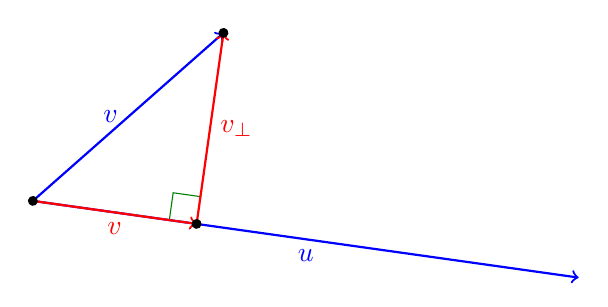
\begin{tikzpicture}[scale=0.7,rotate=-8]
      \draw[draw=green!50!black] (3,0.5) -- (2.5,0.5) -- (2.5,0);
      \draw[->, thick, blue](0,0) -- node[left]{$\vect{v}$} (3,3.5);
      \draw[->, thick, blue](0,0) -- node[below]{$\vect{u}$} (10,0);
      \draw[->, thick, red] (0,0) -- node[below]{$\vect{v}_{\coll}$} (3,0);
      \draw[->, thick, red] (3,0) -- node[right]{$\vect{v}_{\bot}$} (3,3.5);
      \draw[fill](0,0) circle [radius=2.25pt];
      \draw[fill](3,0) circle [radius=2.25pt];
      \draw[fill](3,3.5) circle [radius=2.25pt];
    \end{tikzpicture}
  \end{center}
  To show that such a decomposition exists, let
  \begin{equation*}
    \vect{v}_{\coll} = \proj_{\vect{u}}(\vect{v}) = \frac{\vect{v}\dotprod \vect{u}}{\vect{u}\dotprod \vect{u}}\, \vect{u},
  \end{equation*}
  and define $\vect{v}_{\bot} = \vect{v}-\vect{v}_{\coll}$. By
  definition, {\eqref{projection}} is satisfied, and
  $\vect{v}_{\coll}$ is a scalar multiple of $\vect{u}$. We must show
  that $\vect{v}_{\bot}$ is orthogonal to $\vect{u}$. For this,
  we verify that their dot product equals zero:
  \begin{eqnarray*}
    \vect{v}_{\bot }\dotprod \vect{u}
    &=& \vect{v}\dotprod \vect{u}-\frac{\vect{v}\dotprod \vect{u}}{\vect{u}\dotprod\vect{u}}\,\vect{u}\dotprod \vect{u} \\
    &=& \vect{v}\dotprod\vect{u}-\vect{v}\dotprod \vect{u}\\
    &=& 0.
  \end{eqnarray*}
  To show uniqueness, suppose that {\eqref{projection}} holds and
  $\vect{v}_{\coll}= k \vect{u}$.  Taking the dot product of both
  sides of {\eqref{projection}} with $\vect{u}$ and using
  $\vect{v}_{\bot }\dotprod \vect{u}=0$, this yields
  \begin{equation*}
    \begin{array}{ll}
      \vect{v}\dotprod \vect{u} & = ( \vect{v}_{\coll}+\vect{v}_{\bot }) \dotprod \vect{u} \\
                                & =  k\vect{u} \dotprod \vect{u} + \vect{v}_{\bot} \dotprod \vect{u} \\
                                & = k \norm{\vect{u}} ^{2},
    \end{array}
  \end{equation*}
  which requires
  $k =\vect{v}\dotprod \vect{u} / \norm{\vect{u}} ^{2}$.  Thus there
  can be no more than one such vector $\vect{v}_{\coll}$. Since
  $\vect{v}_{\bot}$ must equal $\vect{v}-\vect{v}_{\coll}$, it follows
  that there can be no more than one choice for both
  $\vect{v}_{\coll}$ and $\vect{v}_{\bot}$, proving their uniqueness.
\end{proof}

\begin{example}{Decomposition into components}{decomposition-into-components}
  Decompose the vector $\vect{v}$ into $\vect{v}=\vect{a}+\vect{b}$
  where $\vect{a}$ is parallel to $\vect{u}$ and $\vect{b}$ is
  orthogonal to $\vect{u}$.
  \begin{equation*}
    \vect{v} = \begin{mymatrix}{r} -5\\3\\-5 \end{mymatrix},\quad
    \vect{u} = \begin{mymatrix}{r} 1\\2\\-2 \end{mymatrix}.
  \end{equation*}
\end{example}

\begin{solution}
  We can let $\vect{a}=\vect{v}_{\coll}$ and $\vect{b}=\vect{v}_{\bot}$
  as in the proof of Theorem~\ref{thm:decomposition-into-components}.
  Then
  \begin{equation*}
    \vect{a} ~=~ \vect{v}_{\coll}
    ~=~ \func{proj}_{\vect{u}}\paren{\vect{v}}
    ~=~ \frac{\vect{v}\dotprod \vect{u}}{\vect{u}\dotprod \vect{u}}\, \vect{u}
    ~=~ \frac{11}{9}\, \begin{mymatrix}{r} 1\\2\\-2 \end{mymatrix}
    ~=~ \begin{mymatrix}{r} 11/9\\22/9\\-22/9 \end{mymatrix}
  \end{equation*}
  and
  \begin{equation*}
    \vect{b} ~=~ \vect{v}_{\bot}
    ~=~ \vect{v}-\vect{v}_{\coll}
    ~=~ \begin{mymatrix}{r} -5\\3\\-5 \end{mymatrix}
    - \begin{mymatrix}{r} 11/9\\22/9\\-22/9 \end{mymatrix}
    ~=~ \begin{mymatrix}{r} -56/9\\5/9 \\-23/9 \end{mymatrix}.
  \end{equation*}
\end{solution}
